\section{Introduction}

This document consists of describing different use cases considered in the project to show the overall functionalities of the system (Figure \ref{Fig-1})and the data flow between different modules. 
\begin{figure}[htbp]
\begin{center}
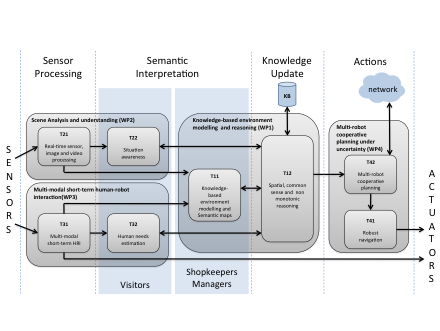
\includegraphics[height=10cm]{ArchitectureCoachesDF}
\caption{Architecture and data flow }
\label{Fig-1}
\end{center}
\end{figure}

\section{Use Cases}
In Task 5.2 of work package WP5, we develop different use cases for demonstration. 
\subsection{Scenario 1: Advertising and informing with simple interaction} 
\subsubsection{Use case 1.1: simple interaction and advertising} 
The use case adopted consists of a smart advertisement mission. The robots receive point of interests and plan to visit these points and announce the appropriate advertising according to the location. The points of interests should be focused on populated area and group detection. The robots should detect group of peoples, move toward this group, select a person to interact with and propose an appropriate advertisement according to the location and the interest expressed by the person. The robots should show a semantic map with appropriate shops with a path to head the shops. This use case illustrate the results developed in tasks T21, T22, T11, T12, T42, T41. 

The objective of this use case is to measure some performance indicators : percentage of good group detection for tasks T21 and T22 ; good expressiveness and message languages for T12 and map expressiveness T11 ; safe navigation and percentage of good advertisements according to the location. 

\subsubsection {Use case 1.2: Informing and guiding}
This use case consists in rendering scenario 1 more complexe by introducing the escorting and guiding services. The robot should guide the person to the destination, bu minting a permanent interaction during the escort or the guide. The customers should follow the robot to destination and the robot should adapt their behavior to the customers moving and behaviors.  The robots should be able to understand the abandon of the customers. This aspect allows us to assess the performance of  tasks T31 of estimating the need of the human. The human can also express their need via the multi-modal interface (Task T32).

The objective of this use case is to measure the same performance indicators as in scenario 1 but also the performance of tasks T31, T32 on the percentage of good need estimation. 

\subsection {Scenario 3: cooperation between robots}
Thee objective of this scenario is to extend scenario 2 to a multi-robot system. In this scenario, we develop a use case to show the ability of robots to cooperate and to share tasks. 
\subsubsection{Use case 3.1: guiding many people with many robots in the same building}
In this use case, we extend  scenario 2 to different persons to guide or escort to different destinations. The robots should, in a decentralized way, share tasks (person or group to guide) and develop a coordinated strategy to assist all of them, to delegate a task if any unexpected event during the assistance and to inform the other robots about other persons to assist. The other aspect we present in this use case is the ability of robots to share space. 
The objective of this use case is to evaluate the performance of task 4.2.

\subsubsection{Use case 3.2: guiding many people from one building to another}
To this end,  we consider a use case  of guiding a person from one building to another where one robot guide the customer to the exit of building 1 and then  assist him to reach the building 2 where the second robot wait him and guides him to the destination. 
The objective of this scenario is to evaluate the tasks of WP4 and task T21. 

\subsection{ Scenario 4 : detecting abnormal events}
\subsubsection*{Use case 4.1: Lost objects}
This use case consists of assessing the modules developed in WP2 in terms of perception. To this end, we consider a use case where external cameras detect object at a location (Task T21), the robot should evaluate if the  object is at a right or wrong location and generate an event (task T22) and the module of task T12 generates a task of visiting the location where the object is located. The robot moves towards the object and send a picture to an operator. 
The objective is mainly based on evaluating image processing task (T2.1).
\subsubsection*{Use case 4.1: Abnormal activities}
This use case is mainly based on evaluating the human activities and assessing the situation. To this end, we consider the detection of some abnormal activities such as 
 the motionless of a customers, the robot moves toward the person and then interact with him to better assess his needs. The rest of interaction scenarii will be developed in use cases 5. Another aspect is to detect a person falling down to send a message for medical assistance if needed. We consider also the waving movement of a person to assess his hesitation and propose him a help;  

This use case allows us to evaluate the performance of tasks in WP2 and in WP3. 

\subsection{Scenario 5 : Short-term interaction and safe navigation}
The examples of this use case is to show different task assistances and interaction between the robot and the customer or the shopkeepers. The functionalities of tasks T3.1, T3.2, T1.2, T1.1, T4.1 and T4.2 will be presented and evaluated. 

\subsubsection {use case 5.1 : Interaction with Customers}
\paragraph*{Customer asks for help carrying his/her bag}
The robot is called by a manager (or by the customer himself) to assist
someone in carrying his/her bag. The robot must reach
the exit of the shop and approach the dedicated loading area. When
in position he looks for the customer and as soon as he establishes
contact, he asks the user to load the bag in the appropriate container.
Once loaded, the robot will ask the customer if he is in a hurry.
If the customer is in a hurry, the robot will proceed at a sustained
speed to the parking lot. In the other case, the robot will leisurely
proceed to the parking lot, proposing intermediate stops to shops
with interesting discounts.

The objective of this use case is to evaluate the performance of tasks T3.1, T3.2 and T4.2.
 
\paragraph*{Use case 5.2: Customer refuses first robot proposal, accepts specific one} Managers have told the robot that he needs to promote a special discount
for a movie. The robot is also aware, in his persistent KB, of the
existence of other secondary discounts. Since there are no people
moving around the robot starts waiting and scanning. As soon as it
sees a suitable user (at the right distance and the right speed),
the robot intercepts the customer and asks him/her if he would be interested
in the special discount for the movie. The user answers that s/he is not interested.
The robot then asks the user to slide his customer card in order to
propose the most appropriate available discount. After reading the
card, the robot finds out that the customer is a woman and that she
has made many purchases in the personal care department. 
So, the robot reasons that the special discount on the facial cream would be of interest
to her. After being informed of the discount, the customer reveals
to be interested and asks the robot for directions to reach the specific
shop. Since not many people are moving around, the robot can safely
guide the customer himself.
The objective of this use case is to evaluate the performance of tasks T3.1, T3.2, T4.2, T1.1 and T1.2.

\paragraph*{Use Case 5.3 : Customer asks for directions in crowded environment} The robot has the objective to inform the customers of a certain few
available discounts. The shopping mall is very crowded and, for safety
considerations, the robot decides it should not move but rather wait
for users to approach. As soon as it detects a user, standing still at
the appropriate social distance, looking at him/her, the robot initiates
conversation and announces the available offers. The user is interested
and asks for directions. Since the robot cannot safely move, it shows
the desired path on his tablet and informs the user that 20m along
the corridor s/he will find another robot for more specific information,
if needed. The human thanks the robot and goes to the next one to
receive further directions.
The objective of this use case is to evaluate the performance of tasks T3.1, T3.2 and T4.1 and T4.2.

\subsubsection {Use case 5.4 : Interaction with Shopkeepers}
\paragraph*{Proposing an ice cream to a child} Manager from local ice cream shop asks robot to inform children about
a special discount. The robot looks around for children. When it detects
one, it approaches him and informs him and his parents of the discount. The child
is passionate about having an ice cream; but before directing him
there, the robot asks for the parent's authorization. Once the parents
agree to allow the child to follow the robot, the robot will proceed
to the ice cream shop. 

The objective of this use case is to evaluate the performance of tasks T3.1, T3.2.

\paragraph*{Use case 5.5 : Shopkeepers ask for carrying bag of customers}
The robot receives messages from a shopkeepers to carry a bag from one location to another. The robot localizes the shop and navigates towards and then asks for the bags to transport and the customers to follow her. The robot should maintain a permanent interaction with the customer and uses the escort function to reach the destination. At the arrival the robot should ask the customers to take its bags and to confirm before leaving him. Without confirmation from the customer, the robot asks the customer to take bags and confirm. After three times, the robot send message to the shopkeeper and come back to the shop for keeping the bags or confirming.

The objective of this use case is to evaluate the performance of tasks T3.1, T3.2, T4.1 T4.2, T1.2 and T1.1.

\subsection {Demonstration}
We propose to use the robots in the Rives De l'Orne Mall of the Caen city, in the collaboration of the city's representative and the Rive de l'Orne manager
\newpage
\section{Test facilities: Collaboration with the Mall Rives de l'Orne}
The test facilities concerns the Mall Rives de l'Orne. � Rive de l�orne � is a new and modern mall at Caen city (France). It is composed of two face-to-face buildings separated by a large main square. At the first floor of the two buildings, there are many shops and restaurants. In the main square, there is a cinema. This space is surrounded by tramway stations and a train station. This mall is visited by more than 100,000 customers every year. In addition to that, several elderly people live in the new apartments at the other floors of the buildings. These people have their habit and there are frequent customers of the mall \ref{mall}. Two meetings have been organized ($23^{th}$ October and $12^{th}$ December 2014)to define the equipments to install in terms of cameras and sensors (RFID) to send some information to robots about shops, the planning of the robot deployment in the mall and some local dissemination actions. A visit of all partners have been organized during the kickoff meeting. 

\begin{figure}[htbp]
\begin{center}
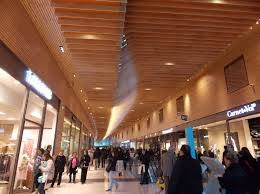
\includegraphics[height=5cm]{InsideRivedelOrne}
\caption{Inside the mall}
\label{mall}
\end{center}
\end{figure}

\begin{figure}[htbp]
\begin{center}
\includegraphics[height=5cm]{MapsRorne}
\caption{The map}
\label{default}
\end{center}
\end{figure}

